\documentclass[12pt]{article}

\title{Research Computing Coursework Report}
\author{James Hughes}

\usepackage{amsmath}
\usepackage{listings}
\usepackage{url}
\usepackage{hyperref}
\usepackage{graphicx}

\lstdefinestyle{style1}{
    basicstyle=\ttfamily\footnotesize,
    breakatwhitespace=false,
    breaklines=true,
    captionpos=b,
    numbers=left,
    numbersep=5pt,
}
\lstset{style=style1}

\bibliographystyle{unsrt}

\begin{document}

\maketitle
\newpage


\section*{Introduction}

Sudoku is a type of simple puzzle, commonly found in the games pages of major UK newspapers.
It first appeared in `The Times' in 2004, but it can be traced back to a series of popular U.S. puzzle books decades earlier, where it was given the title `Number Place'\cite{sudoku}.
For consistency, we propose the following definitions for the game, its rules, and related terms.

\begin{enumerate}
    \item A Sudoku puzzle consists of a $9\times9$ \textbf{grid} where the aim is to fill each of the 81 \textbf{cells} with a single-digit number from 1--9, according to certain rules.
    \item Each puzzle is differentiated by the \textbf{clues} given on the grid to begin with, which restricts the possible solutions. The empty cells (which we denote with a $0$ in the code) must be filled in.
    \item (\textbf{Row condition}) Each row of 9 cells must contain the digits 1--9 exactly once.
    \item (\textbf{Column condition}) Each column of 9 cells must contain the digits 1--9 exactly once.
    \item The grid can be tesselated by 9 square subsets of cells in a $3\times3$ arrangement; these are referred to as the \textbf{boxes}.
    \item (\textbf{Box condition}) Each box must contain the digits 1--9 exactly once.
    \item A grid is \textbf{valid} if its entries satisfy all of the rules above.
    \item A grid is \textbf{solved} if it is valid and contains no cells that are empty.
\end{enumerate}

It should be noted that the arrangement of clues for the starting grid can correspond to zero, one, or multiple solutions.
In 2012, it was proved exhaustively that it is not possible to specify a Sudoku puzzle which has a unique solution if there are less than 17 clues given on the starting grid\cite{17min}.
Therefore, Sudoku puzzles that start with this number of clues represent the `hardest', in the sense that they have the smallest ratio of number of valid solutions to number of all possible solutions.
Such puzzles are used later on to check that the code can handle the toughest cases in a reasonable time.
\section*{Algorithm Selection and Prototyping}
I decided to base my solution on the "templates" method combined with "backtracking" as described on the Wikipedia page about Sudoku solving algorithms \cite{wiki1}.
This is a brute-force method, which relies on the fact that the rules of Sudoku inherently limit the number of possible arrangements of any given digit into nine cells on the grid.
We can see this using a combinatorial argument filling in the $3\times3$ boxes from left-to-right then top-to-bottom: in the first box there are 9 choices, then 6 choices (one row already occupied), then 4 choices (two rows), then 6 choices (one column) and so on.
\[
    \text{Number of possible templates} = 9\cdot6\cdot3\cdot6\cdot4\cdot2\cdot4\cdot2\cdot1 = 46656
\]
The method involves generating all such templates, and then finding the subset of templates that are valid in the context of each digit, with respect to the given clues.
Then, based on the remaining possibilities, we search through all possible combinations of entries of the empty cells.
I opted for a brute-force algorithm since this would be robust; since all possibilities are considered, a solution will be always found so long as it exists.
Moreover, due to the simplicity of the Sudoku-solving problem, even in the worst case (as I discuss later) brute-force does not take too long provided the code is optimised.
In particular, this method has a far smaller search space than backtracking without using templates, and so should be faster, so long as finding the subsets of templates is implemented to be fast.

In my original plan for the software, the first consideration was the memory required to store all the template arrays, which is the most memory demanding data structure in my solution.
Assuming the default NumPy behaviour of storing integer arrays as 64-bit signed integers, this would require $46656\cdot81\cdot8\approx3\cdot10^7$ bytes, or 30MB, which poses no issues.
I decided to store the abstract representation of the grid as a \texttt{np.ndarray} type of shape \texttt{(9, 9)} since this greatly improves the speed of the high number of mathematical operations performed on the grid to find the solution.
However I also anticipated that this could have been subject to change as I started to develop the code.
For this reason, I decided to code the solving part of the code first, and then the next major parts, namely handling the input and output of data, could be coded according to the final choice of representing the grid internally.
It appeared that the two main parts of the code were the solving and then the input and output of data, so I decided that a reasonable modular approach would be to create two separate modules, \texttt{solve.py} and \texttt{data.py} under the package \texttt{sudokutools}.
Finally, I also noted that significant error catching was required somewhere between the input and solve stages, primarily because beyond 'obvious' violations from inputs that do not resemble a sudoku grid, there is the more subtle violation of a grid that does not have a solution, and could therefore cause the solver code to continue indefinitely if not caught.


INSERT DIAGRAM
\section*{Development, Experimentation and Profiling}
I implemented a testing-led development strategy.
This meant that some of the earliest steps that I took in developing any code was orchestrating unit tests to ensure that the next anticipated phase of development was working properly.
The main advantage of this was that it heavily directed my development path, keeping me on the right track.
For instance, in one of my earliest commits (3132ebb) I created the following unit test:

\begin{lstlisting}
    def test_templates():
    count_array = np.zeros((9, 9))
    for template_array in generate_templates():
        count_array += template_array
    count_array_expected = 5184 * np.ones((9, 9))
    assert count_array == count_array_expected
\end{lstlisting}
Besides its purpose for validating my future code, this also ensured that in the next phase of development, I specifically had a function called \texttt{generate\_templates()}, and that its output was of the form of a $9\times9$ NumPy array with binary entries.
This approach during development in general, I already had an idea of what functions I intended to create, and what their inputs and corresponding outputs should look like.

I also made full use of Git to version control my code.
I used three branches: \texttt{main}, \texttt{dev}, and \texttt{test}.
Broadly speaking, I developed the code primarily in the \texttt{dev} branch, and then merged to main once I had code that passed the current testing suite.
The \texttt{test} branch was for experimental features, but I only used this at one point which I mention later; this was when I had an idea that conflicted with my original plan.
I also had a strictly self-enforced commit message style for almost all commits, broadly following the "Convential Commits" guidance \cite{ccommits}.
In particular, while my commit messages weren't as detailed as suggested there, I aimed for a regular structure of a full sentence starting with an imperative term ("Create", "Change", "Remove", "Profile", etc.), and with one of the given "type" words suggested by \cite{ccommits}, such as "Fix", "Test", "Docs", "Build", and "CI".

According to my plan the first development of functional code handled implementing the templates part of the solving method.
This comprised two functions, \texttt{generate\_templates} and later \texttt{find\_valid\_templates}.
The former implemented a generator which iterated through all possible templates. I found that an efficient way of doing this was to:
\begin{itemize}
    \item enumerate each arrangement of a fixed digit (which I labelled 1) on the grid by a list of length 9, with the $i^{th}$ digit of the array giving the column to which the 1 in the $i^{th}$ row belonged - such an arrangement inherently satisfies the row condition;
    \item ensure the column condition is satisfied by only iterating through permutations of (1,...,9);
    \item ensure the box condition is satisfied by finding the remainder of each entry of the array when divided by 3, corresponding to the three boxes on that row, and checking the first, second and third group of 3 entries of the array are individually permutations of (0, 1, 2).
\end{itemize}

Developing the first versions of the template routines that passed the tests was followed by refactoring of some of the functionality.
For instance in one commit, the way that \texttt{find\_valid\_templates} checked whether any of the 8 remaining digits' clues conflicted with a template was massively improved.
Originally, this was done using a double-nested for loop, checking each cell, and making a list of the other digits on each iteration.
This was then changed to initialise the list of \texttt{OTHER\_DIGITS} as a global variable in the module, so that it was only constructed once, saving computational time.
The nested for loops were also substituted for the use of the NumPy method \texttt{isin()} which later became the use of NumPy's \texttt{any()} method.
This refactoring not only improved the computational speed of the routine, but also achieved the same functionality in fewer lines, improving readability of the code.

The first prototype of the solving routine experimentally used a simple for loop to iterate through the Cartesian product of the subsets of templates for each digit, using the \texttt{product} method from \texttt{itertools}.
This was tried before the backtracking algorithm since it only required a very short (11 lines), readable routine, and was therefore worth investigating to see if it was viable.
While this passed the testing suite, even for the most difficult starting grids, it was immediately found to be very slow for any non-trivial starting grid.

At this point, considering how one would solve some of the hardest Sudoku grids by hand illuminated the fact that a further 'smart' filtering of the subsets of templates was possible.
In particular, in some cases the initial clues for a given digit allow certain cells to be filled by using the fact that they are a kind of 'fixed point' in the subset of templates, that is, in all valid templates, a certain cell is always occupied by that digit, but this isn't given as an explicit clue.
The simplest case of this is when, say, the top left box does not contain a clue for the digit 7, but the other boxes occupying the top row and the left column, do.
In turn, in many cases this allows us to fill in some cells on the grid with certainty, so we can re-use the \texttt{find\_valid\_templates()} routine on the updated grid, repeat this for all digits in a loop.
This experimental feature was developed in the \texttt{refine\_valid\_templates()} method in the \texttt{test} branch, with a loop halting when the grid is no longer updated after iterating through all digits.
The advantage of the feature is that it also uses a brute-force style approach, but in each instance the search space is very small (assuming the initial clues included at least one of each digit 1--9, the set of templates for a given digit to search through is no more than 5184).
In some of the starting grids with more clues, this routine was found to be sufficient to solve the grid entirely.

After this, it was clear that the backtracking part of the solving algorithm was necessary to solve---in a reasonable time-frame---the grids that were still fairly empty after the new template step.
In the first prototype of this routine, a nested list of generators was instantiated at the start of the routine, with each generator representing the possible digits that could occupy the corresponding cell.
A NumPy array \texttt{search\_positions} was used to store the coordinates of the cells that were empty, and thus formed part of the backtracking procedure.
The variable \texttt{search\_idx} was initialised at zero, and used to keep track of the current location of the backtracking procedure on the grid.
At each stage, this variable was incremented by 1 to move to next cell in the search, when a valid entry was found for the current cell, and decreased by 1 to move to the previous cell, when all options for the current cell were exhausted.
Once this variable reached the maximum (the number of coordinate pairs in \texttt{search\_positions}) and the entries of the search cells constituted a valid grid, the backtracking was halted.

Next, the data handling part of the code package was developed.
This module has two functions, \texttt{read\_grid} and \texttt{write\_grid}.
Their development began with simple functionality that effectively handled the valid input cases where the arguments they received were in the expected format.
For instance, the first prototype of \texttt{read\_grid} simply read the specified file line-by-line, building a nested list of characters in each line that was a digit character, and returning this as a NumPy array.
This worked for text files formatted in the prescribed way, but lacked robustness, raising errors in the face of the most minor violations to this format.

I then implemented extensive error catching starting with the data handling routines in \texttt{data.py}.
This was appropriate since this module contains front-end functions where the input is more likely to created by a user who could make a mistake such as:
\begin{itemize}
    \item Formatting the grid incorrectly
    \item Specifying the wrong filepath, or similarly not using a .txt file.
    \item Specifying a non-existing file.
\end{itemize}
The error catching was developed to handle such transgressions.
The approach taken was to take a lenient approach in the case of a badly formatted grid; so long as the text file contained exactly 9 lines that contained any number of digit characters, and each of these contained exactly 9 digit characters, the input file was accepted.
This meant that input files unambiguously specifying a Sudoku grid were accepted, despite any bad formatting with the characters "|", "+" and "-", and also reduced the complexity of the code as these decorative characters were not checked.
In the case of any of the other violations above, an informative string was printed explaining the error, and an empty Sudoku grid was returned.

At this point the \texttt{sudokutools} had been fully constructed with all necessary functionality, and steps such as testing and documentation had been implemented.
The next step was to profile the code using \texttt{line\_profiler}, whose outputs were exported as .txt files in a separate \texttt{prof} directory.
This was done in the \texttt{dev} branch of the repository.
The profiling was focused on the solving functions, which were the main bottleneck in the end-to-end solution of a grid specified by an input .txt file, to be outputted to the terminal or a .txt file.
In particular, the function \texttt{solve\_backtrack} was profiled with input grids of a variety of difficulties, since this function also called all of the other backend solving functions.
Regardless of the starting grid, it was found that the largest percentage (between 75.5\% and 99.5\%) of time was spent on the lines calling the \texttt{find\_valid\_templates()} and \texttt{refine\_valid\_templates()} functions.
Further profiling of the latter revealed that most of its own computational time was spent calling the former function, which was therefore the main bottleneck in producing a solution in a short amount of time.

In order to optimise the \texttt{find\_valid\_templates()} function, the main change was to represent the full space of templates as a 3D NumPy array of shape \texttt{(46656, 9, 9)} rather than as a list of arrays.
Moreover, where before the subsets of valid templates for each digit were stored in a nested list, this was also changed to be a NumPy array of shape \texttt{(9, 46656)}, with each row representing the indices of valid templates for that digit.
This enabled the use of NumPy's \texttt{any()} method; rather than looping through the list of all templates, to find the list of valid templates.
This was compatible with the representation of the grid as a 2D NumPy array itself; the check involved creating two new \texttt{(9, 9)} shaped arrays, representing the locations of the digit of interest, and the 'other digits' in the grid, and then checking that both were compatible with the any given template array by using the \text{any()} method across the 2nd and 3rd axes of the \texttt{ALL\_TEMPLATES} array.

\section*{Validation, Unit Tests and Continuous Integration}

The main form of continuous integration used in this project was via the\texttt{pre\-commit} package \cite{precommit}.
This package enables the developer to specify a file \texttt{.pre-commit-config.yaml} in the root of the repository directory, which determines which 'hooks' to be run every time a commit is attempted.
In this project, the latest (at the time of development) versions of \texttt{Black} \cite{black} and \texttt{Flake8} \cite{flake8} were used in the file, as well as some pre-defined hooks from the \texttt{pre-commit} repository itself.
The hooks imported from \texttt{pre-commit} apply simple checks to all file types, for instance checking that all files have a consistent newline character, including one at the end of the file.
\texttt{Black} is a code formatter, which applies changes to files directly, usually rearranging code so that lines are not too long.
On the other hand, \texttt{Flake8} is a linter which means it only detects changes, but this typically allows it to be more stringent - for this reason it was made to be the final pre-commit hook, so that it could double check the changes made by \texttt{Black}.
The \texttt{Black} and \texttt{Flake8} hooks only applied to Python scripts in the repository, aiming to ensure their compliance to PEP 8 \cite{pep8}, a widely-used style guide for Python.
During the course of the project, it was realised that the two Python hooks were in conflict with eachother in certain instances.
For example, in trying to commit an updated solve.py script, \texttt{Black} was formatting a block of code to look like:
\begin{lstlisting}
    BOX_GRIDS[
        grid_idx,
        3 * (grid_idx // 3) : 3 * (grid_idx // 3) + 3,
        3 * (grid_idx % 3) : 3 * (grid_idx % 3) + 3,
    ] = 1
\end{lstlisting}
However, \texttt{Flake8} was then blocking the commit on the grounds of PEP 8 rules \cite{wspace}. However, this appears to be a misapplication of the PEP 8 guide, which allows spaces around colons when used for slicing.
Subsequently the \texttt{Flake8} hook was modified to include \texttt{args: [--extend-ignore=E203]} to avoid this conflict; \texttt{Black}'s hook was changed to enforce line-lengths of 79 characters for similar reasons (complying with PEP 8 and avoiding conflicts).
Notably, no hook was included to run the test-suite upon each commit.
This would have slowed down development due to the long time taken for the test suite to run, particularly in the early stages of development.
In an ideal project, continuous integration would include automatic running of the test suite upon any merge to the main branch on the remote GitLab repository, and block such a merge if any test failed.

In light of the long time required to run the tests, the test suite was divided into three python scripts under the \texttt{test} directory: one for the data handling module, and two for the grid solving functions, with a separate script for the tests that used the minimal starting clue grids (since these took the longest).
The \texttt{pytest} module was used to run the tests.
There are eleven tests for the \texttt{data} module functions.
To validate the \texttt{read\_grid()} function, one test checks that the correct NumPy array is used when the expected input file format is used.
The rest of the tests handle other cases, such as an input file not in the expected format but can be used to determine a grid, as well as tests that check a helpful error message is outputted when invalid filepaths are given to read.
Similarly, two of the tests for the \texttt{write\_grid()} function are used to check that it correctly handles writing to a file, and outputting to the terminal, while the other three check that invalid inputs such as non-array types, or arrays that are of the wrong shape or data-type, are handled correctly.
In the case of the \texttt{solve} module, the tests are used to check that the routines correctly handle their given inputs.
For instance, the \texttt{check\_grid\_valid()} function is tested twice, checking that it correctly outputs \texttt{True} for a valid grid, and \texttt{False} for an invalid grid.
Most of the other functions have a similar level of testing; little validation in terms of error catching is necessary since these are backend functions whose inputs are from other functions, rather than from users who could misspecify the input.
The main exception to this is the \texttt{solve\_backtrack()} function whose input \texttt{grid} should be verified to ensure that the grid indeed has a solution, to prevent an infinite loop in the runtime.
The testing suite validates this function with six unit tests overall, with one covering the case of a grid with no solution, and the rest covering starting grids with a range of difficulties, including a starting grid that only has nine empty cells, to another that has just one filled cell, to a starting grid antagonistically designed against the backtrack algorithm (see Figure \ref{antagonist_clues})

\begin{figure}[hbt]
    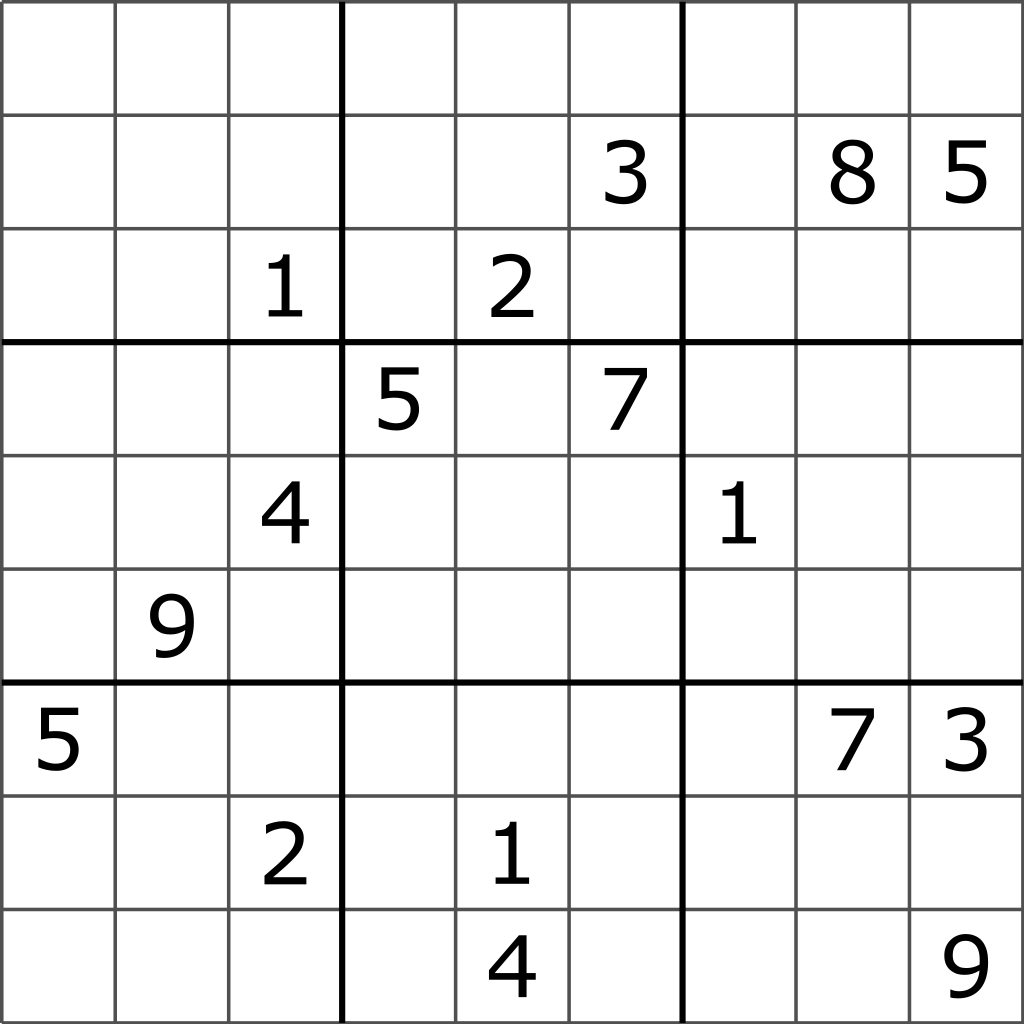
\includegraphics[scale=0.3]{Sudoku_puzzle_hard_for_brute_force.png}
    \caption{A Sudoku puzzle designed to take a long time with the backtracking algorithm \cite{antagonist}.}
    \label{antagonist_clues}
\end{figure}

\section*{Packaging and Usability}

Structure of packages, modularity, refactored code routines, naming

In the project Docker was used to make the code more portable.
A Dockerfile in the repository root directory specifies exactly how to build the Docker image, which starts with a basic image from Docker Hub that has conda already installed \cite{docker}.
It then copies the repository into the image and updates the conda environment using \texttt{environment.yml}.
This is a file which specifies the exact dependencies present in the conda environment used to run the code, allowing for reproducible results, regardless of the user's own conda set-up.
This file was exported from conda using the \texttt{--no-builds} option meaning that it can be used to reproduce the environment on any operating system, so that the repository is portable even if Docker is not used.

The code was also documented using Doxygen \cite{doxygen}.

Error catching

\section*{Summary}

Reasons for software development practices
Extensions, e.g. non-unique solution catching

Lessons learnt?

\bibliography{Biblio}

\end{document}
